


\chapter{Serial Peripheral Interface}

\section{Introduction}

After exploring one for the most fundamental peripherals, the \verb|GPIO|, now we continue for other peripherals.\\ 

We start with SPI: serial peripheral interface, which is a communication protocol which allows sending or retrieving data between a master, and couple of slave devices (such as memory card, connection module such as bleuthooth,$\cdots$)

\subsection{Other Protocols}

There exist other protocol also as shown in, where each protocol has its features, usage, limitation,$\cdots$, Example of such protocols are shown in \autoref{fig:spi:protocol_examples}.

\begin{figure}[h]
\centering
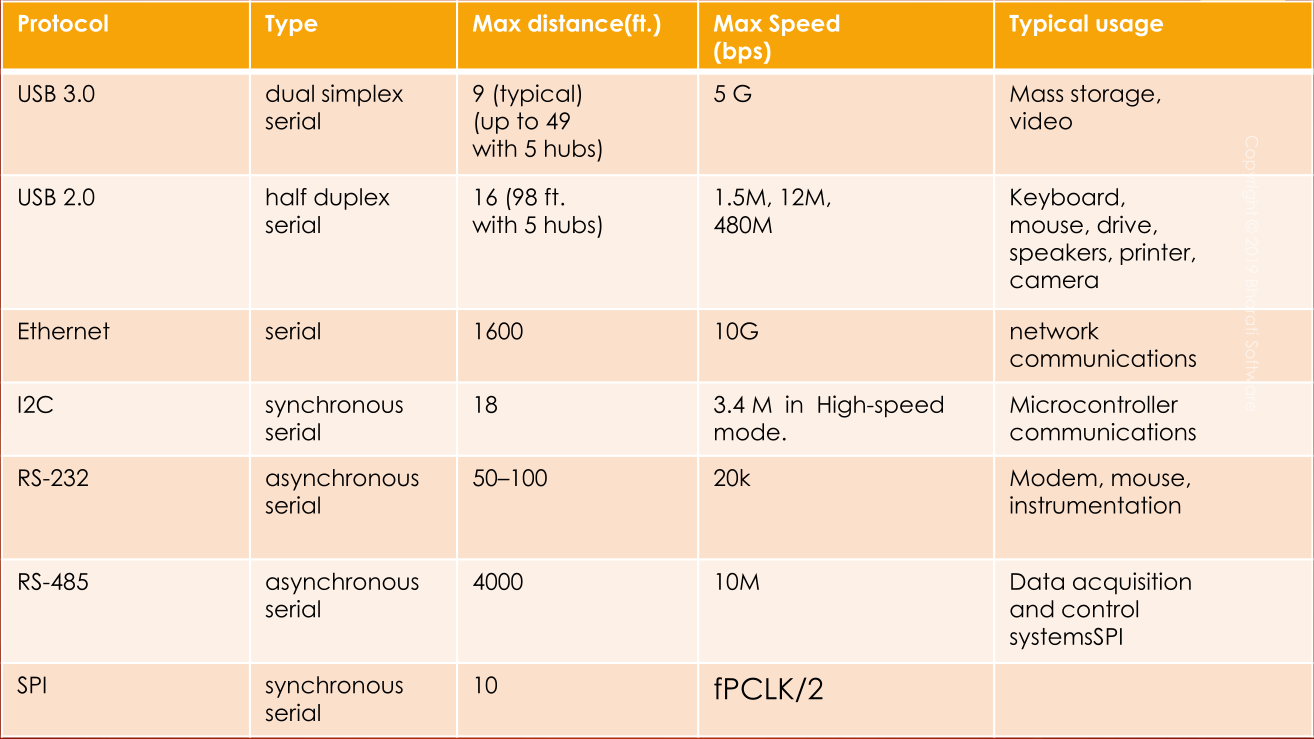
\includegraphics[scale=0.35,frame]{Figures/spi/protocol_examples}
\caption{Communication Protocol Examples}
\label{fig:spi:protocol_examples}
\end{figure}



\begin{itemize}

\item \verb|SPI|: 

	\begin{itemize}
	\item can achieve high speed but with limited distance
	
	\item Usage: gather data from sensor. 
	
	Exampple: fetch some data from seriral flash into the RAM
	\end{itemize}


\item If we take a look at \verb|I2C|:

	\begin{itemize}
	\item it much slower in terms of bps compared to \verb|SPI|
	
	\item but has more features and more complex
	\end{itemize}

\item Now both \verb|SPI| and \verb|I2C| \tbi{are short range serial communication protocol}

	\begin{itemize}
	\item If we want to cover more distance such as home automation, factory,$\cdots$, we need to use other protocols such as \verb|CAN|,\verb|EHTERNET|,$\cdots$
	\end{itemize}

\end{itemize}


\newpage
\section{SPI Bus}

Let's explore the bus details of \verb|SPI| peripherals.

\begin{figure}[h]
\centering
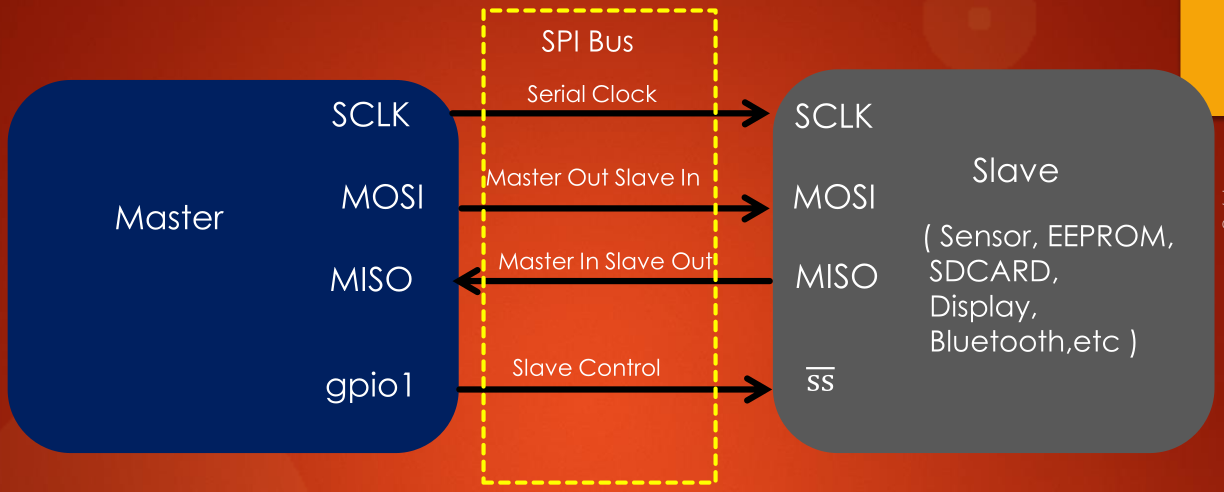
\includegraphics[scale=0.40,frame]{Figures/spi/spi_diagram}
\caption{SPI Bus}
\label{fig:spi:spi_diagram}
\end{figure}

\begin{itemize}

\item MISO: Pin used to trasmit data in slave mode and recieve data in master mode

	\begin{itemize}
	\item In other words, whenever the salve is trasmitting, the master recieve data over this pin
	\end{itemize}

\item MOSI: opposite of MISO, whenever master wants to trasmitt, it uses this pin and the salve receive over this pin

\item SCLK: the clock line. Whenever master and slave want to communicate, the SCLK line will be synchronized with MOSI and MISO line, hence the \verb|SPI| is a \tbi{sychronized protocol}

	\begin{itemize}
	\item The master device has control on the clock line, that is only the master generate the clock and the slave receive it only
	
	\item Slave device doesn't have control on clock line
	\end{itemize}


\item NSS or SS: to select which slave device in case we have more thant 1 salve, the master wants to communicate

	\begin{itemize}
	\item This line doesn't carry any data at all
	\end{itemize}

\end{itemize}

\subsection{Devices}

Now suppose we have some MCU and some slave device and we want to use \verb|SPI|. An important condition is that the slave device should also support \verb|SPI| protocol, otherwise we can't use it even if the MCU support \verb|SPI|.\\

Another important point is about communication. Whenever a master want to communicate with a salve device, the $\mathrm{1}^\mathrm{st}$ thing master does is \tbi{select the salve device}, and that's done by connecting a \verb|GPIO| line of the master to the \verb|SS| pin of the slave, and then pull this line to ground, as shown in \autoref{fig:spi:slave_selection}.


\begin{figure}[h]
\centering
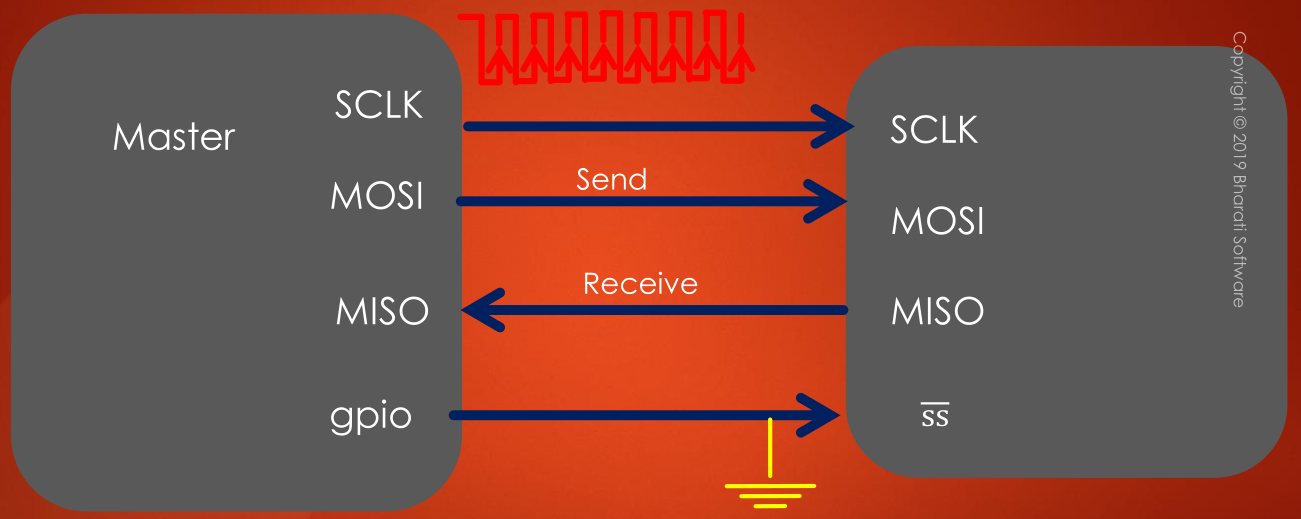
\includegraphics[scale=0.40,frame]{Figures/spi/slave_selection}
\caption{Slave Selection}
\label{fig:spi:slave_selection}
\end{figure}

\subsection{Minimal SPI Bus}
\label{sub:min_spi_bus}

Suppose we have a communcation scenraio between 1 master and \tbi{1} slave, and the \tbi{slave only recieve}. In this case, the \verb|SPI| protocol can use only 2 lines: 1 for the clock signal, and 1 for the data transfer using \verb|MOSI| line (see \autoref{fig:spi:spi_diagram}). The \verb|SS| pin should be pulled ground, and could be done internally via the configuration of the slave. We don't need a \verb|GPIO| line from master to slave as in \autoref{fig:spi:slave_selection} since we have 1 slave only.

So in other words, the \verb|SPI| protocol should not always use the 4 lines, it depends on the situation we have.


\newpage
\section{SPI Mechanism}

Now let's move to the data communication mechanism in which \verb|SPI| uses to transfer data between master and a slave device.

\verb|SPI| uses the concept of \textit{shift register}, that is in each clock cyclce, the data will be shifted from source to destination bit by bit.\\

\autoref{fig:spi:spi_data_transfer} show an example of 8 bit data trasnfer from master to slave, for 2 clock cycles.


\begin{figure}[h]
\centering
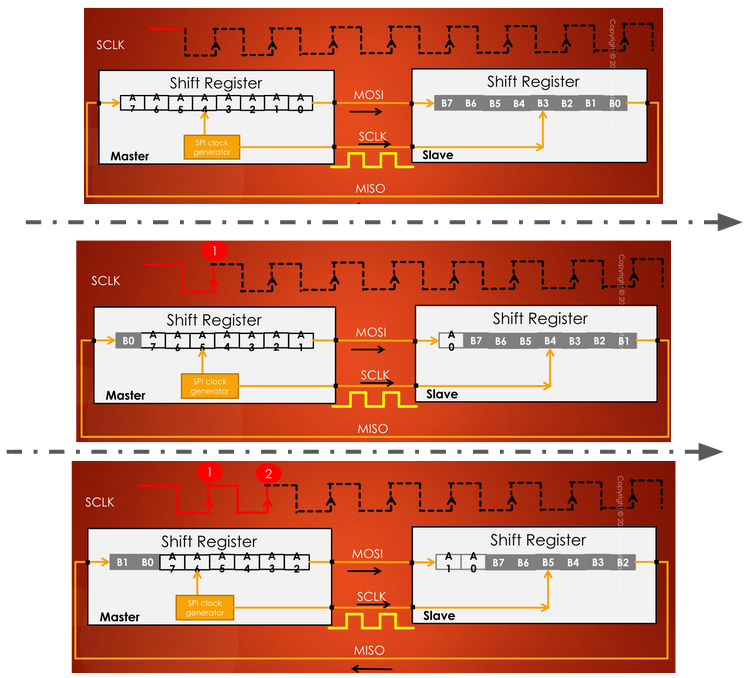
\includegraphics[scale=0.65,frame]{Figures/spi/spi_data_transfer}
\caption{SPI data transfer for 2 clock cycles}
\label{fig:spi:spi_data_transfer}
\end{figure}

\newpage
\section{SPI Configuration}

Now let's explore some different configurations about the \verb|SPI| protocol.\\


\underline{Full Duplex:} that is when we are transmitting, we can also receive

\begin{figure}[h]
\centering
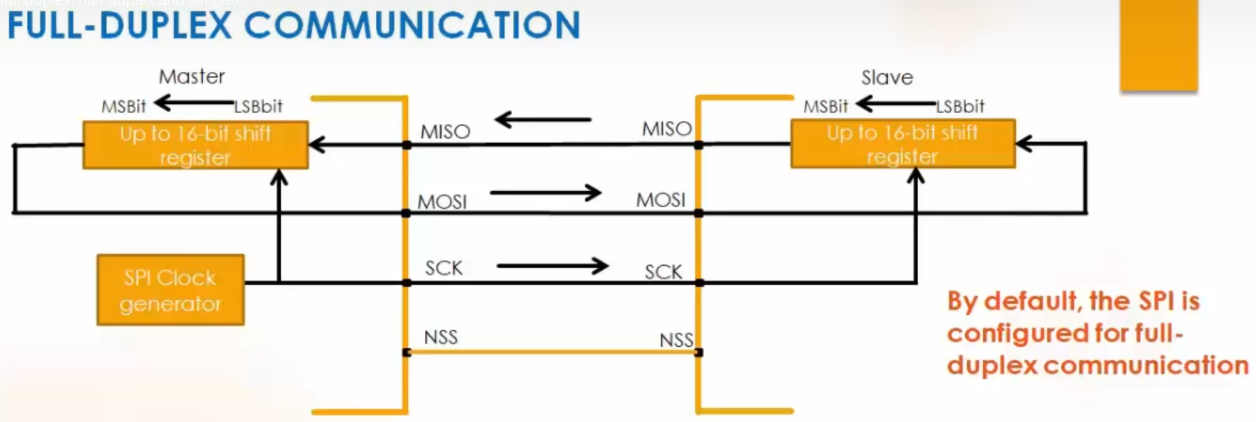
\includegraphics[scale=0.35,frame]{Figures/spi/spi_full_duplex}
\caption{SPI in full duplex mode}
\label{fig:spi:spi_full_duplex}
\end{figure}

\begin{itemize}

\item Slave and master are linked using 2 unidirectional lines between \verb|MOSI| and \verb|MISO| pins.
	
\item Data is shifted synchronously on clock edges provided by the master
	
\end{itemize}

\underline{Half Duplex:} We are either transmitting or receiving at a single clock cycle 

\begin{figure}[h]
\centering
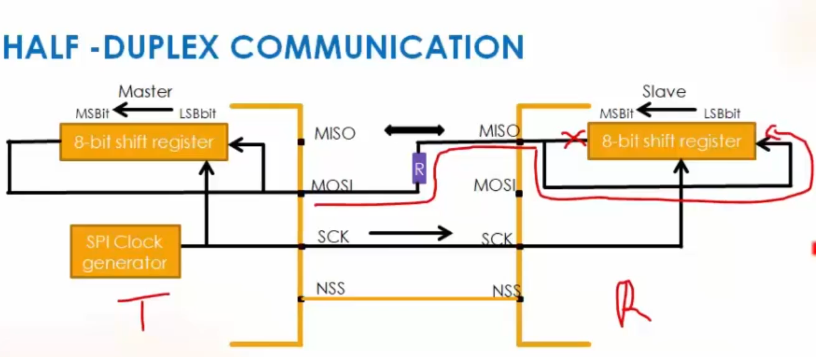
\includegraphics[scale=0.40,frame]{Figures/spi/spi_half_duplex}
\caption{SPI in half duplex mode}
\label{fig:spi:spi_half_duplex}
\end{figure}

\begin{itemize}


\item A single line is used to link shift registers of the master and slave. By this we can save 1 pin and use it for other purposes

\item In the example of \autoref{fig:spi:spi_half_duplex}, the master is transmitting and the slave is receiving

	\begin{itemize}
	\item \verb|MOSI| is connected to \verb|MISO| since master is transmitting
	
	\item We need a resistor between the 2 pins of typical value of 1 kohm
	\end{itemize}


\end{itemize}

\newpage
\underline{Simplex mode:} the devices can only transmit or receive, and the other line is disconnected and ignored

\begin{figure}[h]
\centering
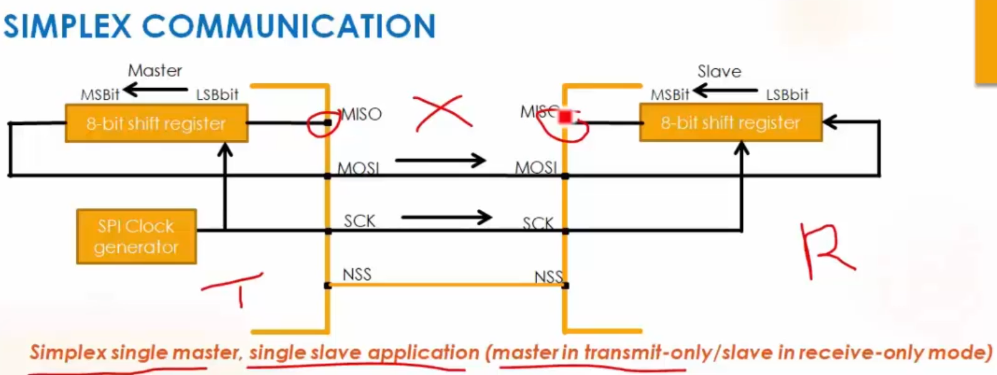
\includegraphics[scale=0.40,frame]{Figures/spi/spi_simplex}
\caption{SPI in simplex mode}
\label{fig:spi:spi_simplex}
\end{figure}

\begin{itemize}

\item In example of \autoref{fig:spi:spi_simplex}, the master is transmitting and the slave is receiving

\item Thus the \verb|MOSI| lines are connected and the \verb|MISO| lines are disconnected 

	\begin{itemize}
	\item Since we are in simplex, the salve will never transmitt, it only receive the whole time
	\end{itemize}


\end{itemize}

\uti{Simplex Mode} \todo{Simplex Mode Configuration}

\begin{itemize}

\item \textit{In the course, it is said that the configuration for simplex mode are in the same as in full duplex}

\item \textit{I didn't understand why, to be seen later}

\item \textit{Source: MCU driver part 1 course, section 32, video 126}

\end{itemize}

\newpage
\section{SPI Block Diagram}

Now we move to the block diagram of \verb|SPI|, provided in the reference manual, section 28.3.

\newpage
\section{SPI Summary}

\begin{itemize}

\item \verb|SPI| is a serial and sychronized protocol

\item \verb|SS| line should be pulled to ground before any communication start

\item \verb|SPI| can use only 2 lines (\ref{sub:min_spi_bus}): 1 for clock and 1 for data transfer


\end{itemize}




